\documentclass[xcolor=dvipsnames]{beamer} 
\usecolortheme[named=Blue]{structure} 
\usetheme[height=10.5mm]{Rochester} 
\setbeamertemplate{items}[ball] 
\setbeamertemplate{blocks}[rounded][shadow=true] 
\setbeamertemplate{navigation symbols}{} 
\usepackage{bm}
\usepackage{listings}
\usepackage{rotating}
\usepackage{graphicx}
\usepackage{multirow}
\usepackage{hyperref}
\usepackage{textcomp}
\usepackage{upquote}
\usepackage[absolute,overlay]{textpos}
\newenvironment{reference}[2]{%
  \begin{textblock*}{\textwidth}(#1,#2)
      \footnotesize\it\bgroup\color{red!50!black}}{\egroup\end{textblock*}}
%\graphicspath{ {/home/ben/PhD/Armidale_Updates/2014_03_14/Figures/} }
\begin{document}

%%% New plan for this module:
%%% we all use Git on the command line and view GitHub in our web browsers
%%% clone and commit via HTTPS
%%% Workflow plan:
%%%
%%% Create repo in web browser
%%% Authenticate on cmd line
%%% Clone
%%% Add files
%%% Edit
%%% git add
%%% git commit
%%% branch and revert to previous version with check out


%%% Getting on the command line in various OS's

%%% MS Windows -> Start Menue -> Powershell
%%% Mac OS -> Finder -> terminal
%%% GNU+Linux users -> application launcher (will vary depending on GUI) -> terminal 


\begin{frame} %1
% \frametitle{Addressing Common Challenges in Spatial Modeling of Ecologies and Environments}
\begin{center}
\textbf{\huge Version Control with Git}\\
\end{center}

\begin{figure}
%\includegraphics[width = 0.35\textwidth]{/home/ben/Intro_to_R/GitHub_Slides_Source/Images/GitHub-Mark-120px-plus.png}
\begin{columns}

\begin{column}{3.3cm}
\begin{center}
\begin{figure}

\includegraphics[width = 0.9\textwidth]{/home/ben/Intro_to_R/Introductory_Slides_Source/Images/R_logo.png}
\end{figure}
\end{center}
\end{column} 

\begin{column}{3.3cm}
\begin{center}
\begin{figure}

\includegraphics[width = 0.9\textwidth]{/home/ben/Intro_to_R/GitHub_Slides_Source/Images/Git-Icon-1788C.pdf}
\end{figure}
\end{center}
\end{column} 

\begin{column}{3.3cm}
\begin{center}
\begin{figure}

\includegraphics[width = 0.9\textwidth]{/home/ben/Intro_to_R/GitHub_Slides_Source/Images/GitHub-Mark_Big.pdf}
\end{figure}
\end{center}
\end{column} 

\end{columns}
\end{figure}

\small Ben R. Fitzpatrick\\
\tiny PhD Candidate, Statistical Science, Mathematical Sciences School, Queensland University of Technology
\newline
\begin{columns}
\begin{column}{3cm}
\tiny 0000-0003-1916-0939
\end{column}
\begin{column}{3cm}
\tiny github.com/brfitzpatrick/
\end{column}
\begin{column}{3cm}
\tiny @benrfitzpatrick
\end{column}
\end{columns}
\end{frame}

\begin{frame}
\frametitle{Version Control Software}
Have you ever put numbers or dates at the end of a file name to keep different versions of it? 
\begin{itemize} 
\item If yes then you have already used version control!
\newline
\newline
\end{itemize}

Have you ever used track changes and comments to take turns editing a  MS Word document with one or more others?
\begin{itemize}
\item If yes then you have collaboratively edited a file!
\newline
\newline
\end{itemize}

Version Control Software: 
\begin{itemize} 
\item formalizes these concepts
\item can do a lot of the organisational work for you
\item makes reverting to previous versions without losing work easy 
\end{itemize}
 
\end{frame}

\begin{frame}
\frametitle{Benefits of Using Version Control Software}
\begin{block}{Version Control for Working Solo}
\begin{itemize}
\item Easy to revert to previous versions of a file without loosing any of the subsequent revisions
\item Simple to create multiple versions of a file and edit them in parallel with the option combine them again at a later date
\end{itemize}
\end{block}

\begin{block}{Benefits of Distributed Version Control for Collaborating}
\begin{itemize}
\item Greatly simplifies your life
\item Different contributors can edit different versions of the same files concurrently 
\item Tools exist to systematically combine versions of the same file from different contributors
\item Time stamped record of all changes from all contributors - if someone breaks something you can revert to when it last worked and work forward to discover the bug 
\end{itemize}
\end{block}

\end{frame}

\begin{frame}
\frametitle{Why Git?}
\begin{itemize}
\item Git is free and open source
\newline
\newline
\item Git is available for most operating systems
\newline
\newline
\item Git is Distributed and Fast
\newline
\newline
\item Two major code hosting services (GitHub \& BitBucket - both with free plans) support version control with Git
\end{itemize}
% \tiny $^1$ Google Code will close in 2016 as they have deemed it is no longer necessary given success of BitBucket and GitHub
\end{frame}

\begin{frame} 
\frametitle{Git is Distributed Version Control}
Distributed Version Control means that:
\begin{itemize}
\item every contributor has a copy of the entire database up to when they copied it (all revisions of all files)
\newline
\item two or more contributors can work on the files in their copy of the database independently then combine their modifications systematically at a later date
\newline
\newline
\end{itemize}
Results is a fast and flexible version control system: \begin{itemize}
\item contributors can work independently offline connecting to the server sporadically to submit their changes
\newline
\item most operations are performed locally (on individual contributors' computers) so less waiting for the server
\end{itemize}

\end{frame} 

\begin{frame}
\frametitle{Why Git on the Command Line?}
\begin{itemize}
\item Makes discrete components of the workflows obvious.
\newline
\item This in turn will enable you to migrate easily to one of the many GUIs at a later date should you so desire (and these are generally well documented and easy to learn yourself esp. GitHub's GUI)
\newline
\item The workflows we will practise today function identically at MS Windows, MacOS and GNU+Linux command line interfaces.
\end{itemize}
\end{frame}

\begin{frame} 
\frametitle{Plan for this Module}
\framesubtitle{Part 1}
\begin{block}{Version Control for Working Alone}
\begin{enumerate}
\item Set up Git on your laptop to communicate with the GitHub servers
\item Create a local \textbf{clone} of a \textbf{remote repository}
\item Make some changes to the files in your local copy of the repository
\item \textbf{commit} these changes to your copy of the history of revisions of these files 
\item \textbf{push} these changes to your local copy of the repository to the remote copy on the GitHub servers
\item make some more changes
\item revert to a previous version of a file in this repository safely by \textbf{checking out} an previous \textbf{commit} to a new \textbf{branch} of the revision history of that file
\end{enumerate}
\end{block}
\end{frame}

\begin{frame} 
\frametitle{Plan for this Module}
\framesubtitle{Part 2}
\begin{block}{Collaborating with Git \& GitHub}
\begin{enumerate}
\item fork the repository of a fellow course attendee
\item clone your fork of their repository creating a local copy on your hard drive
\item edit one of their files in your local copy of their repository
\item commit your changes to your local copy of their repository
\item summit a pull request - requesting the repository owner merge your changes with their branch of the repository
\item watch the merge process on your fellow course attendee's computer 
\item switch roles and repeat
\end{enumerate}
\end{block}

\end{frame}

\begin{frame}
\frametitle{Creating a Repository on the GitHub Servers}
\framesubtitle{Log into the GitHub Web Service \& Create a New Repository}
\begin{center}
\begin{figure}
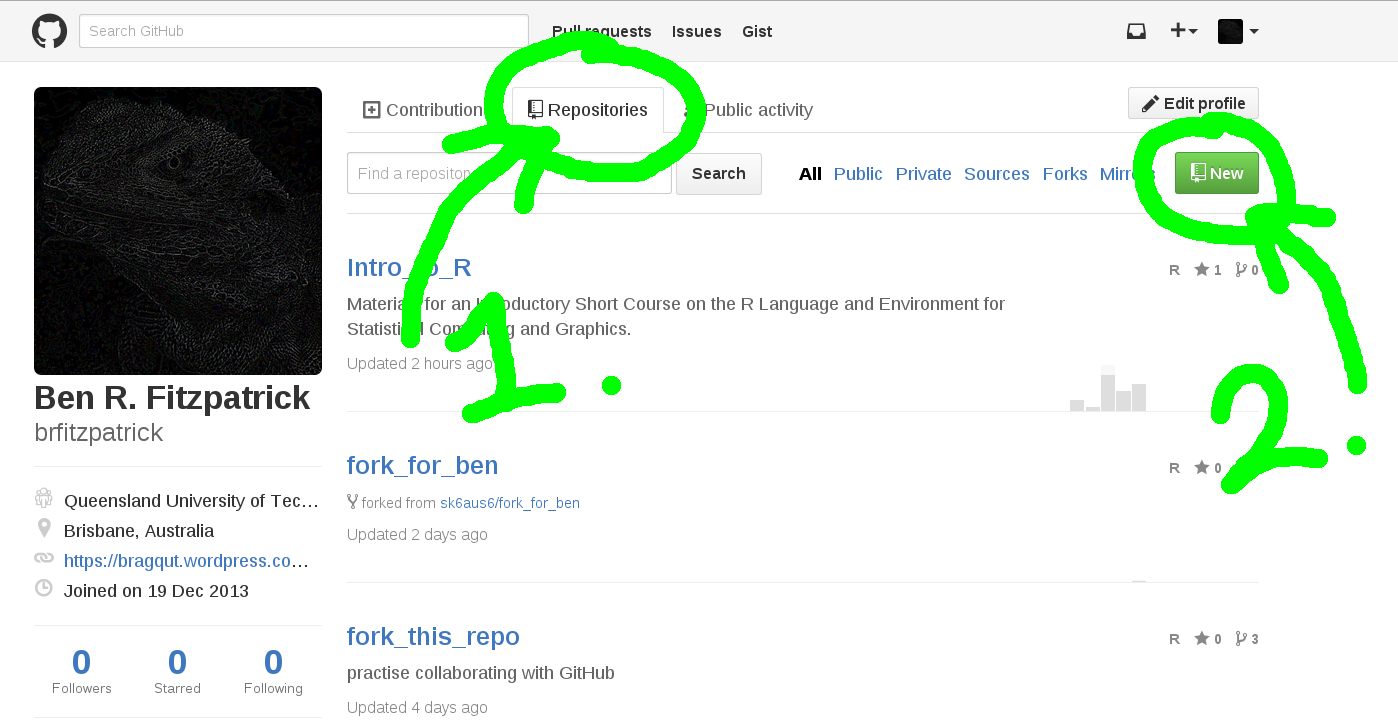
\includegraphics[width = \textwidth]{/home/ben/Intro_to_R/GitHub_Slides_Source/Images/New_Repo_1.png}
\end{figure}
\end{center}
\end{frame}

\begin{frame}
\frametitle{Creating a Repository on the GitHub Servers}
\framesubtitle{Complete the Details}
\begin{center}
\begin{figure}
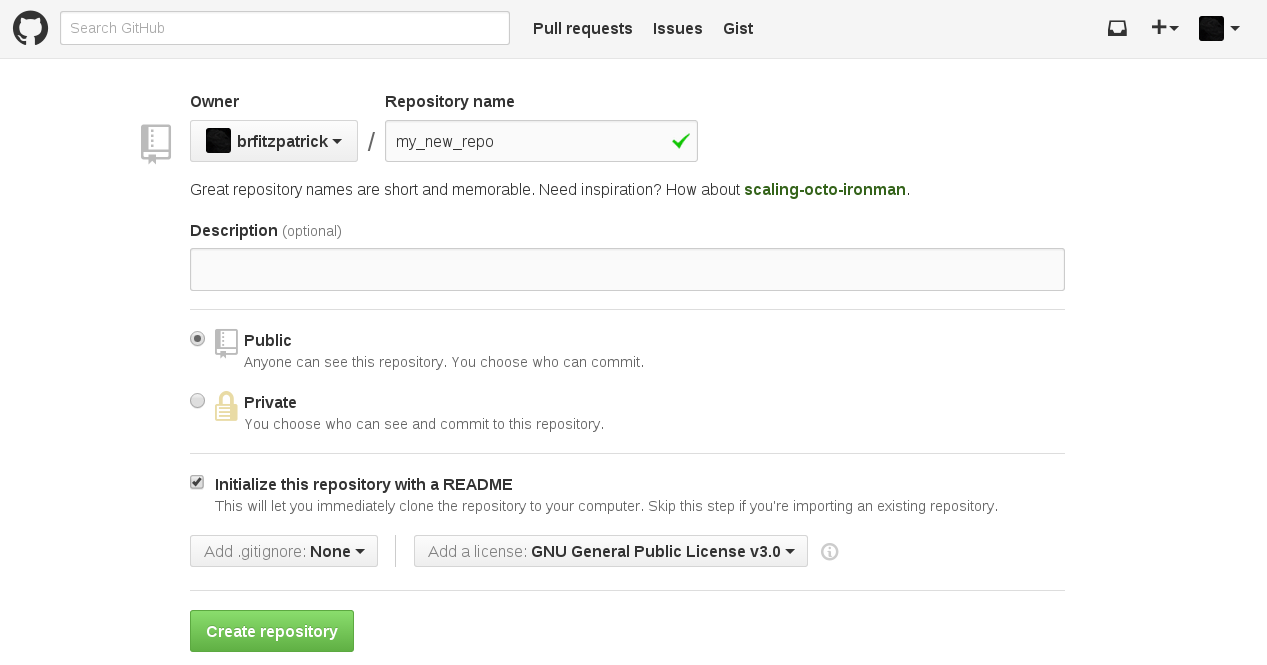
\includegraphics[width = \textwidth]{/home/ben/Intro_to_R/GitHub_Slides_Source/Images/New_Repo_2.png}
\end{figure}
\end{center}
\end{frame}

\begin{frame}
\frametitle{Creating a Repository on the GitHub Servers}
\framesubtitle{View your New Repository}
\begin{center}
\begin{figure}
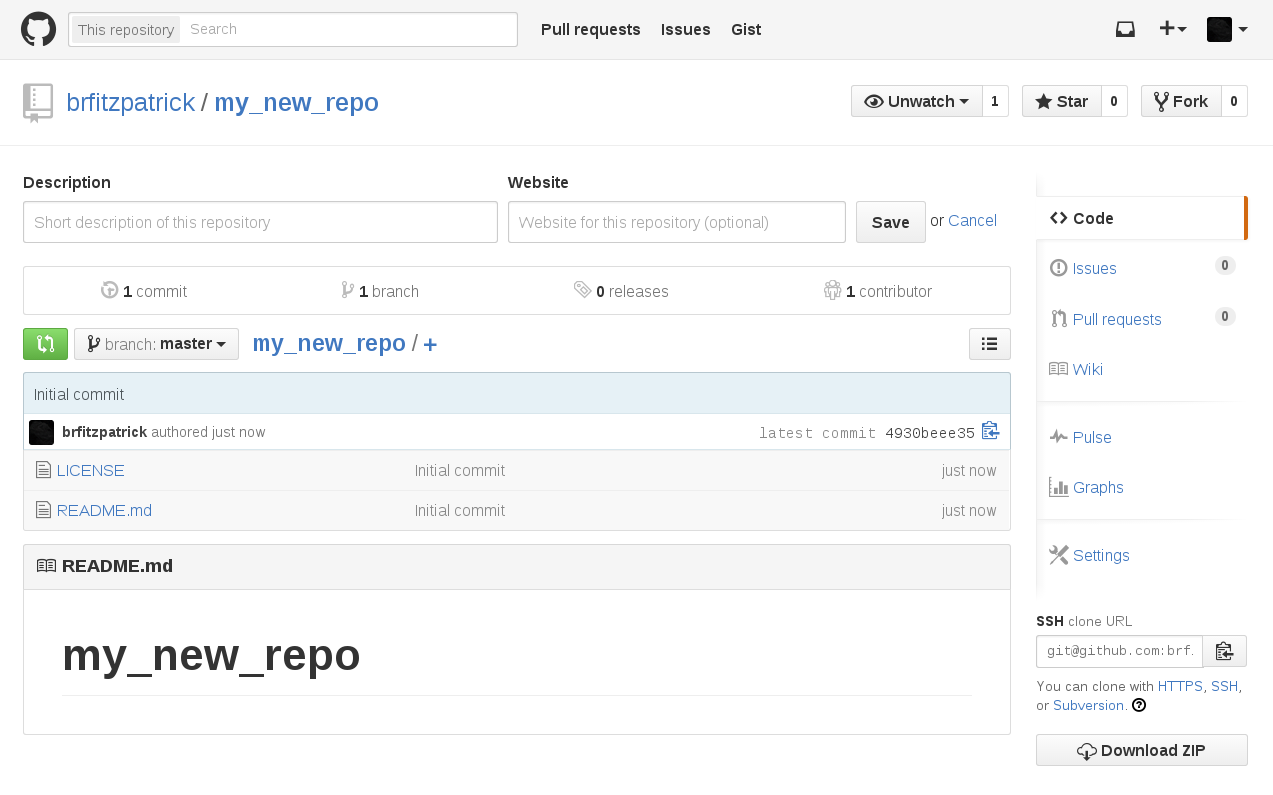
\includegraphics[width = \textwidth]{/home/ben/Intro_to_R/GitHub_Slides_Source/Images/New_Repo_3.png}
\end{figure}
\end{center}
\end{frame}

\begin{frame}
\frametitle{Cloning your new Repository to your Hard Drive}

First, create a folder on your Hard Drive in which to store your Git Repositories.  
\newline
\newline
We are now going to use the Git command line application to `clone' your new repository from the GitHub servers to your hard drive.
\newline
\newline
Git uses distributed version control so a Git `clone' is a complete copy of the entirity of the repository i.e.\begin{itemize}
\item all the files
\item the entire history of snapshots of files states created each time you commit modifications to the respository
\newline \end{itemize}
Being a distributed version control system Git doesn't require you to be connected to the GitHub servers to work on your files and commit them to your local clone of the repository.

\end{frame}

\begin{frame}
\frametitle{Git on the Command Line}
Accessing a command line interface in your OS of choice
\begin{columns}

\begin{column}{3.3cm}

\begin{center}
MS Windows\\
Open a `PowerShell'

\begin{figure}
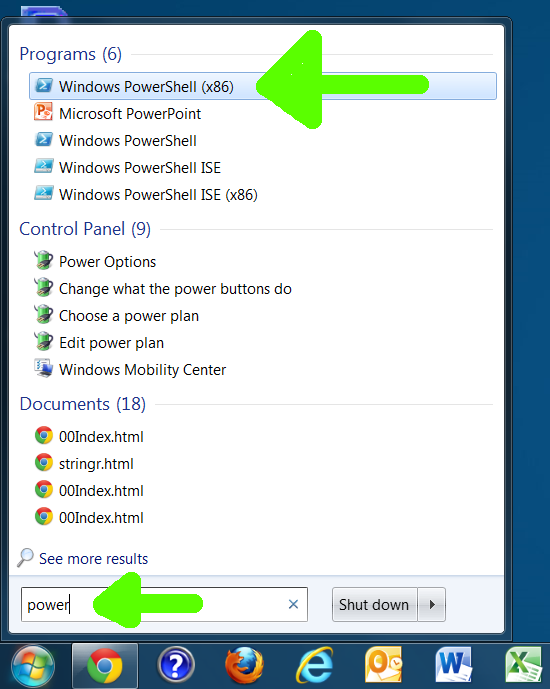
\includegraphics[width = \textwidth]{/home/ben/Intro_to_R/GitHub_Slides_Source/Images/Git_on_MS_Windows_Powershell/Powershell.png}
\end{figure}

\end{center}

\end{column} 

\begin{column}{3.3cm}
Mac OS X \& later\\
Open a `Terminal'
\begin{center}
\begin{figure}
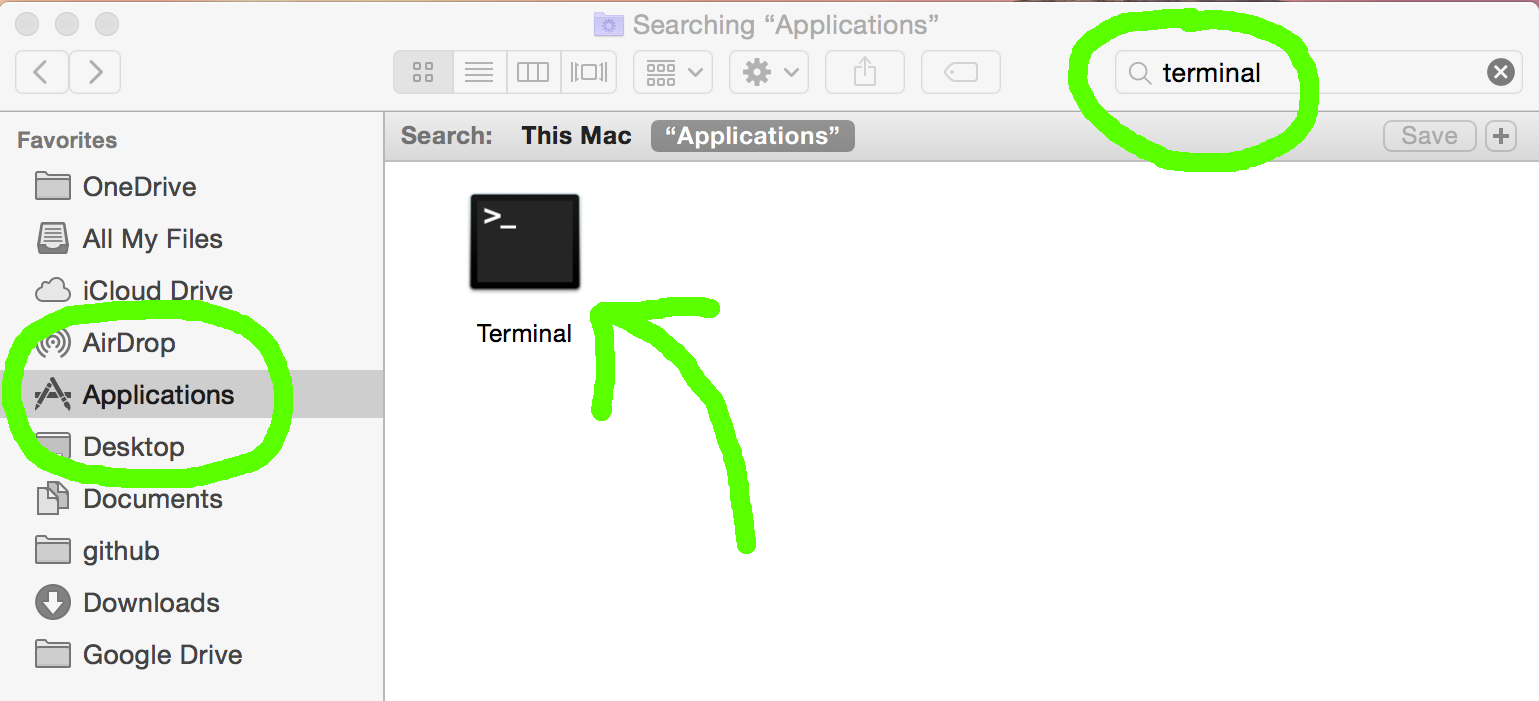
\includegraphics[width = \textwidth]{/home/ben/Intro_to_R/GitHub_Slides_Source/Images/Git_on_MacOS_Terminal/MacOS_Launch_Terminal_Annotated.png} %% insert MacOS Screenshot here
\end{figure}
\end{center}
\end{column} 

\begin{column}{3.3cm}

\begin{center}
GNU+Linux\\
Open a `Terminal'

\begin{figure}
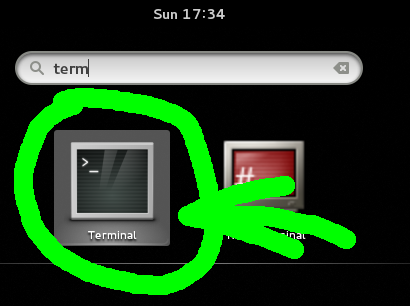
\includegraphics[width = \textwidth]{/home/ben/Intro_to_R/GitHub_Slides_Source/Images/Git_on_GNU_Linux_Terminal/Launch_Terminal.png}
\end{figure}

\end{center}

\end{column} 

\end{columns}
\end{frame}

\begin{frame}
\frametitle{Accessing a command line interface in MS Windows}
\framesubtitle{Open a `PowerShell'}
\begin{center}
\begin{figure}
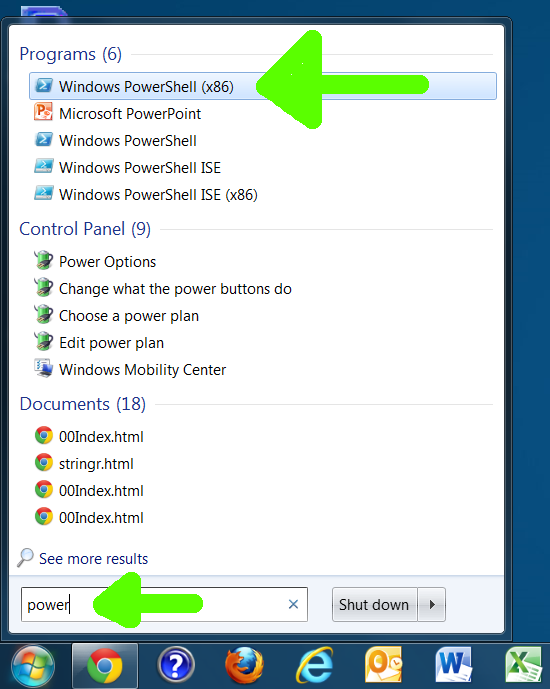
\includegraphics[height = 0.9\textheight]{/home/ben/Intro_to_R/GitHub_Slides_Source/Images/Git_on_MS_Windows_Powershell/Powershell.png}
\end{figure}
\end{center}
\end{frame}

\begin{frame}
\frametitle{Accessing a command line interface in MacOS}
\framesubtitle{Open a `Terminal'}
\begin{center}
\begin{figure}
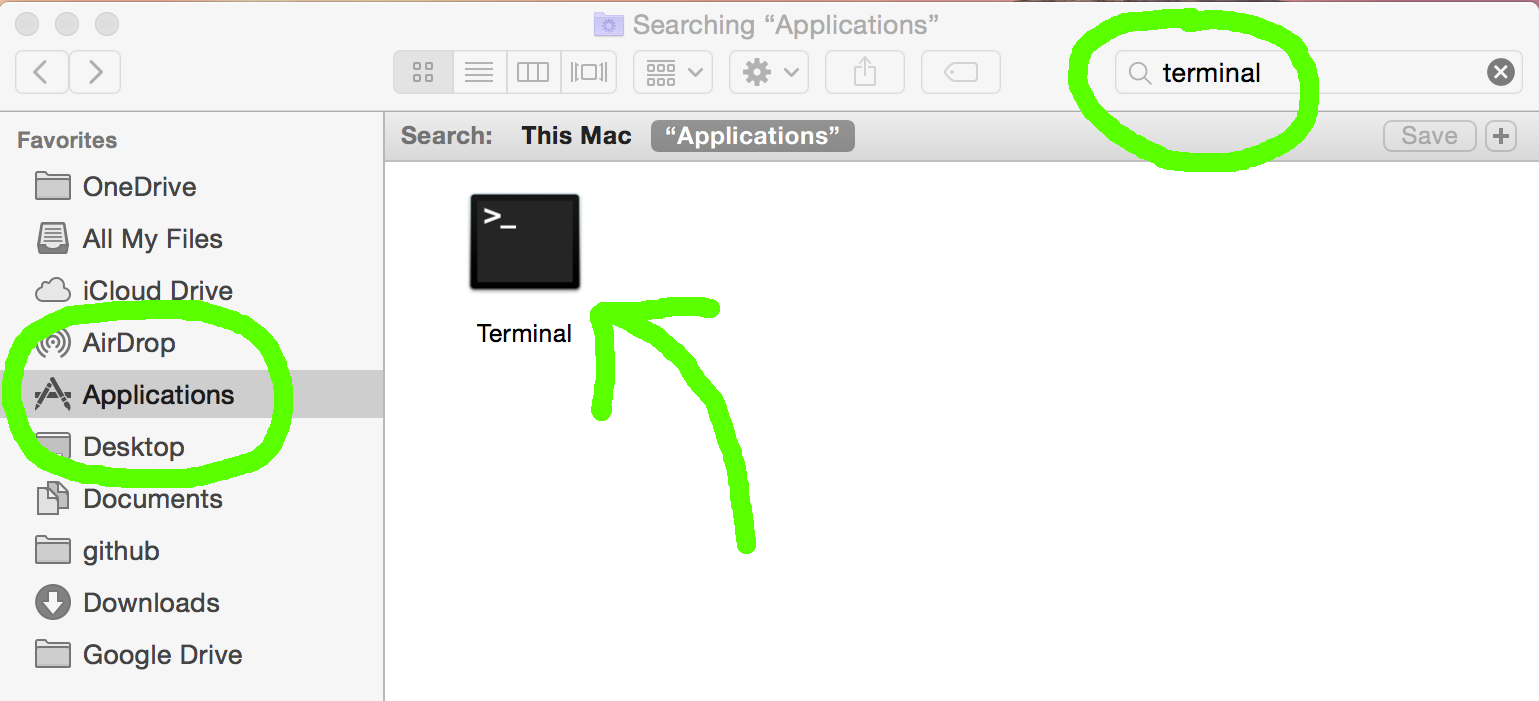
\includegraphics[width = \textwidth]{/home/ben/Intro_to_R/GitHub_Slides_Source/Images/Git_on_MacOS_Terminal/MacOS_Launch_Terminal_Annotated.png} 
\end{figure}
\end{center}
\end{frame}

\begin{frame}
\frametitle{Accessing a command line interface from GNU+Linux}
\framesubtitle{Open a `Terminal'}
\begin{center}
\begin{figure}
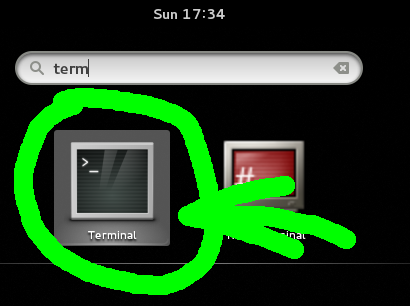
\includegraphics[height = 0.9\textheight]{/home/ben/Intro_to_R/GitHub_Slides_Source/Images/Git_on_GNU_Linux_Terminal/Launch_Terminal.png}
\end{figure}
\end{center}
\end{frame}

\begin{frame}[fragile]
\frametitle{Configuring Git for the first time}
\begin{block}{All Users}
\begin{lstlisting}
> git config --global user.name "Your Name"
> git config --global user.email you@mail.com
\end{lstlisting}
\end{block}
\end{frame}

\begin{frame}[fragile]
\frametitle{Configuring Git for the first time}
\framesubtitle{Choosing a Global Editor}
The global editor is used to write your commit messages.
\newline
\newline
Default is Vim but Vim is a little heavy on keyboard short cuts for some...
%Many of the below can also function as an IDE for authoring R code if you prefer one of them to RStudio.
\newline
\newline
Other Options: \begin{itemize}
\item Notepad (available on all Windows PCs)
%\item TextEdit (available on most Macs)
\item Atom: \url{https://atom.io/docs/v1.0.0/getting-started-installing-atom}
\item Sublime: \url{http://www.sublimetext.com/2}
\item TextMate: \url{http://macromates.com/download}
\item Emacs: \begin{verbatim} sudo apt-get install emacs \end{verbatim} 
\end{itemize}

\end{frame}

\begin{frame}[fragile]
\frametitle{Configuring Git for the first time}
\url{https://help.github.com/articles/associating-text-editors-with-git/}
\begin{block}{Set a Text Editor of your choice as the global editor}
%# TextEdit:
%> git config --global core.editor 'open -t -n -W'
You'll need relevant the text editor installed for the below to work:
\begin{lstlisting}
# Notepad:
> git config --global core.editor notepad.exe
# Atom:
> git config --global core.editor "atom --wait"
# Sublime:
> git config --global core.editor "subl -n -w"
# TextMate:
> git config --global core.editor "mate -w"
# Emacs:
> git config --global core.editor "emacs"
\end{lstlisting}
\end{block}

\end{frame}

\begin{frame}[fragile]
\frametitle{Cloning Your Repository from the GitHub Servers}

Set the working directory to the location on your hard drive to which you would like the repository cloned then list the files and folders present at that location:

\begin{block}{Powershell Users}
\begin{lstlisting}
> C:
> cd C:\Users\username\Documents\GitHub_Repos\
> dir 
\end{lstlisting}
\end{block}

\begin{block}{Terminal Users}
\begin{lstlisting}
> cd /home/username/Documents/GitHub_Repos
> ls 
\end{lstlisting}
\end{block}
\end{frame}

\begin{frame}
\frametitle{Copy HTTPS URL to use when cloning repository}
\begin{center}
\begin{figure}
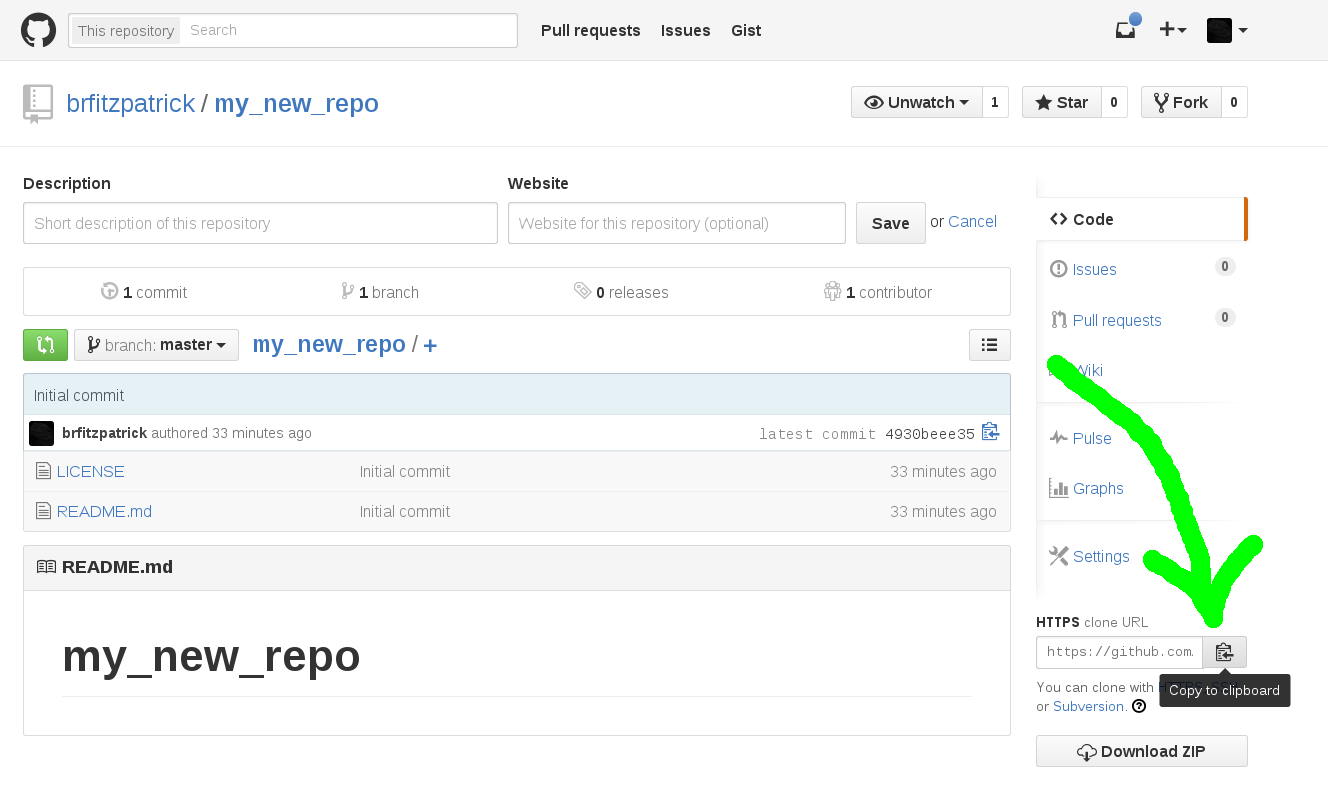
\includegraphics[width = \textwidth]{/home/ben/Intro_to_R/GitHub_Slides_Source/Images/Clone_Repo_1.png}
\end{figure}
\end{center}
\end{frame}

\begin{frame}[fragile]
\frametitle{Clone your Repository: GitHub Servers $\rightarrow$ your Hard Drive}
Use the HTTPS URL you copied earlier:\\
\begin{center}
\begin{figure}
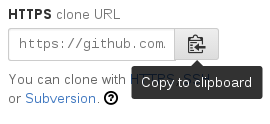
\includegraphics[width = 0.5\textwidth]{/home/ben/Intro_to_R/GitHub_Slides_Source/Images/HTTPS_Clone.png}
\end{figure}
\end{center}

\begin{block}{All Users}
\begin{lstlisting}
> git clone https://github.com/.../my_new_repo
  .git
> cd ./my_new_repo/
> ls
> git status
\end{lstlisting}
\end{block}

If you look in your file browser you'll be able to see your newly cloned repository as a directory in the location to which you cloned it.

\end{frame}

\begin{frame} 
\frametitle{Git}
\framesubtitle{The Four States of Files in a Directory Git is Tracking}
Files in a directory which you are version controlling with Git can exist in one of four states:
\begin{itemize}
\item \textbf{committed} data stored in the database for the associted repository
\item \textbf{modified} local copy of a file (in your working directory) is different to the most recent version of that file stored in the database for the associted repository i.e. you have changed something but not comitted the changes (yet)
\item \textbf{staged} the local copy of a file which you have modified is marked to be added to the database in the next commit snapshot you send to the database
\item \textbf{untracked} Git is not recording revisions to this file 
\end{itemize}
\end{frame}

\begin{frame} 
\frametitle{Git}
\framesubtitle{Basic Git Workflow}
\begin{enumerate}
\item you add files to or modify existing files in your local copy of the repository
\newline
\item you stage these modified files to be committed to the database for the repository
\newline
\item you perform a commit which takes the files as they were when staged and stores a snapshot of them in the database for the repository
\newline
\item you push the changes recorded in this commit to your remote copy of this repository on the GitHub servers
\end{enumerate}
\end{frame}

\begin{frame}[fragile]
\frametitle{Git}
\framesubtitle{Adding New Files}
\begin{enumerate}
\item Open your favourite program for authoring R code (e.g. RStudio)
\newline
\item Create an new R script (it can be very short) 
\newline
\item Save your R Script in the local version of your repository
\end{enumerate}

\end{frame}

\begin{frame}[fragile]
\frametitle{Git}
\framesubtitle{Adding New Files to the List of Tracked Files}

\begin{block}{}
\begin{lstlisting}
> git status
On branch master
Your branch is up-to-date with 'origin/master'.
Untracked files:
  (use "git add <file>..." to include in what 
will be committed)
\end{lstlisting}
\end{block}

We have to tell Git that we want it to track the changes we make to this new file

\end{frame}

\begin{frame}[fragile]
\frametitle{Git}
\framesubtitle{Adding New Files to the List of Tracked Files}

We have to tell Git that we want it to track the changes we make to this new file
\begin{block}{}
\begin{lstlisting}
> git add filename.R
> git status
On branch master
Your branch is up-to-date with 'origin/master'.
Changes to be committed:
  (use "git reset HEAD <file>..." to unstage)

	new file:   filename.R
\end{lstlisting}
\end{block}
We can still change our mind about adding the file to the repository at this stage quite easily.

\end{frame}

\begin{frame}[fragile]
\frametitle{Git}
\framesubtitle{Commiting Changes}
Once you're ready to `commit' this change to the permanent record of changes in this repository we make a `commit'
\begin{block}{}
\begin{lstlisting}
> git commit
[master 311acfb] Initial Commit of some R code.
1 files changed, 0 insertions(+), 0 deletions
(-) create mode 100644 filename.R
\end{lstlisting}
\end{block}
You will be prompted to write a short description of the changes you are committing - these become invaluable as your project grows and if you are collaborating.\\
Once you've written a commit message, save it and close the text editor you used to write it.\\
You should see confirmation of the commit immediately below the git commit line.
\end{frame}

\begin{frame}[fragile]
\frametitle{Git}
Now that you've commited some changes to your local clone of the repository this local version will be ahead of the version on the GitHub Server
\begin{block}{}
\begin{lstlisting}
> git status
On branch master
Your branch is ahead of 'origin/master' by 1
commit.
 (use "git push" to publish your local commits)
\end{lstlisting}
\end{block}
Seeing as we are all currently connected to the internet, it's a good time to `push' these changes to GitHub server (`origin/master' in the default setup) to bring the remote copy of this repository up to date.
\end{frame}

\begin{frame}[fragile]
\frametitle{Git}
\framesubtitle{Pushing changes to local repository to remote repository}
\begin{block}{}
\begin{lstlisting}
> git push
Counting objects: 3, done.
Delta compression using up to 8 threads.
Compressing objects: 100\% (2/2), done.
Writing objects: 100\% (3/3), 353 bytes | 0 bytes/s, done.
Total 3 (delta 0), reused 0 (delta 0)
To git@github.com:brfitzpatrick/my_new_repo.git
   4930bee..99d61f1  master -> master
\end{lstlisting}
\end{block}
If you return to the page for your repository on the GitHub website and refresh the page you should see your most recent commit listed on the repository page.
\end{frame}

\begin{frame}[fragile]
\frametitle{Git}
\framesubtitle{Pushing changes to local repository to remote repository}
Furthermore, now that we have `pushed' our most recent changes our local copy of the repository to the remote copy of the repository on the GitHub servers these two versions of the repository will be identical
\newline
\begin{block}{}
\begin{lstlisting}
> git status
On branch master
Your branch is up-to-date with 'origin/master'.
nothing to commit, working directory clean
\end{lstlisting}
\end{block}
\end{frame}


%\begin{frame}[fragile]
%\begin{block}{the whole process}
%\begin{lstlisting}
%> git clone git@github.com:brfitzpatrick/my_new_repo.git
%Cloning into 'my_new_repo'...
%remote: Counting objects: 4, done.
%remote: Compressing objects: 100\% (3/3), done.
%remote: Total 4 (delta 0), reused 0 (delta 0), pack-reused 0
%Receiving objects: 100\% (4/4), 12.12 KiB | 0 bytes/s, done.
%Checking connectivity... done.
%> cd my_new_repo/
%> touch filename.R
%> emacs filename.R 
%> git add filename.R
%> git commit
%[master 99d61f1] My first commit of some R code.
% 1 file changed, 2 insertions(+)
% create mode 100644 filename.R
%> git push
%Counting objects: 3, done.
%Delta compression using up to 8 threads.
%Compressing objects: 100\% (2/2), done.
%Writing objects: 100\% (3/3), 353 bytes | 0 bytes/s, done.
%Total 3 (delta 0), reused 0 (delta 0)
%To git@github.com:brfitzpatrick/my_new_repo.git
%   4930bee..99d61f1  master -> master
%\end{lstlisting}
%\end{block}
%\end{frame}

\begin{frame} 
\frametitle{Undoing Things Safely}
\framesubtitle{Checking out Previous Commits to a New Branch}
To revert to a previous version of a file that you have a `snapshot' of from a previous `commit'\\
Click on the file name on the GitHub website and click the `History' button:
\newline
\newline
Provided we have commited all changes to the file then it is safe to use the checkout command which will overwrite the file in the current local working directory with the file from the previous `commit'.
\newline
\newline
You can think of commits a bit like save points, if we have two we can move between them but if we load an old save without first making a current save we will loose the unsaved changes
\end{frame}

\begin{frame}[fragile]
\frametitle{Git}
\framesubtitle{Undoing Things Safely}
List existing branches of current repository:
\begin{block}{}
\begin{lstlisting}
git branch
\end{lstlisting}
\end{block}
then, choose a commit you'd like to go back to, copy the corresponding SHA from the history tab on the website and checkout this previous commit to a new branch called `testing', here abbreviated to $(SHA = 58...a44)$:
\begin{block}{}
\begin{lstlisting}
> git checkout -b testing 58...a44
  Switched to a new branch 'testing'
> git branch
    master
  * testing
\end{lstlisting}
\end{block}

\end{frame}

\begin{frame}[fragile]
\frametitle{Git}
\framesubtitle{Undoing Things Safely}
Now if you open your .R file you'll see that you have a previous version of the file without the new changes.\\
Next up we'll make some changes to the version of this file on the branch `testing' so that it will diverge from the version on the branch `master'.\\
Once again check you're on the branch called `testing'
\begin{block}{}
\begin{lstlisting}
> git branch
\end{lstlisting}
\end{block}
then make some changes on testing branch by editing the version of the file currently in your working directory then save those changes, add them, commit them and push them `upsteam' to server:
\begin{block}{}
\begin{lstlisting}
> git push --set-upstream origin testing
\end{lstlisting}
\end{block}

\end{frame}

\begin{frame}[fragile]
\begin{itemize}
\item Now if you check the website your repository should now have two branches.
\newline
\newline
\item We also know that each branch contains a slightly different file now.
\newline
\newline
\item Next we'll `merge' your changes from 'testing' back into the `master' branch.
\end{itemize}
\end{frame}


\begin{frame}[fragile]
To merge into a branch we must be on that branch:\\
\begin{block}{}
\begin{lstlisting}
> git checkout master
\end{lstlisting}
\end{block}

Now we will attempt to merge `testing1' into current branch (master)
\begin{block}{}
\begin{lstlisting}
> git merge testing1
  Auto-merging filename.R
  CONFLICT (content): Merge conflict in 
  filename.R
  Automatic merge failed; 
  fix conflicts and then commit the result.
\end{lstlisting}
\end{block}
\end{frame}

\begin{frame}[fragile]
\frametitle{Resolving a Merge Conflict with a Merge Tool}
\begin{block}{}
\begin{lstlisting}
git mergetool

This message is displayed because 'merge.tool' 
is not configured.
See 'git mergetool --tool-help' or 'git help
 config' for more details.
'git mergetool' will now attempt to use one
of the following tools:
meld opendiff kdiff3 tkdiff xxdiff 
...
emerge vimdiff
Merging:
filename.R
\end{lstlisting}
\end{block}
\end{frame}

\begin{frame}[fragile]
\frametitle{Resolving a Merge Conflict with a Merge Tool}
\begin{block}{}
\begin{lstlisting}
Normal merge conflict for 'filename.R':
  {local}: modified file
  {remote}: modified file
Hit return to start merge resolution tool
(meld): 
\end{lstlisting}
\end{block}
\end{frame}

\begin{frame}[fragile]
\frametitle{Resolving a Merge Conflict with a Merge Tool}

Demonstrate \textbf{Meld}
%Insert Screen shot of \textbf{Meld} in action

\end{frame}

%\begin{frame}[fragile]
%\frametitle{Git}
%\framesubtitle{Undoing things}
%%%One way to safely experiment with past versions of a file is to create a new `branch' in the repository in which to do so
%\newline
%\newline
%branches are separate lines of development of the same files
%\newline
%\newline
%let's make a new `testing3' branch checking out a previous version of the file filename.R\\
%\begin{lstlisting}
%> git checkout 99d61f19d85ae7aec691feb81ca8aef59f6a0719 -b testing3

%> git push --set-upstream origin testing3
%\end{lstlisting}
%we can then move between branches with the checkout command
%\begin{lstlisting}
%> git checkout master

%> git checkout testing3
%\end{lstlisting}
%\end{frame}

%\begin{frame}[fragile]
%  \frametitle{Merging Branches}
%To merge the `master' and `testing3' branches
%\begin{block}{}
%\begin{lstlisting}
%> git checkout master
%> git merge testing3
%\end{lstlisting}
%\end{block}

%if you get a merge conflict use a mergetool to resolve the conflict\\
%(you should have one installed by default from when you installed Git)

%\begin{block}{}
%\begin{lstlisting}
%> git mergetool
%\end{lstlisting}
%\end{block}
%\end{frame}

%\begin{frame}[fragile]
%  \frametitle{Merging Branches}
%
%\begin{block}{once you have resolved the conflict}
% \begin{lstlisting}
%  > git add filename.R
%  > git commit
% \end{lstlisting}
% \end{block}

%\begin{block}{finally you can delete your testing branch if you're done with it}
% \begin{lstlisting}
%  > git branch -d testing3
% \end{lstlisting}
% \end{block}
%\end{frame}

%\begin{frame}
%\frametitle{Branching}
%
%%%'Branching means you diverge from the main line of development and continue to do work without messing with that main line.'

%Every project starts with the default `master' branch
%%%%you can then make a new branch e.g. a `testing' branch which will initially be the same as the `master' branch at the point in time at which you create it
%you switch to another branch by `checking out' that branch
%you can then commit changes to this branch without alterning the `master' branch i.e. you could develop some new feature without risking breaking the functionality of the master branch while you do so
%once your feel your work on the a branch is complete you can `merge' your `testing' branch with the `master' branch

%branching allows for collaboration, various contributors can all make their own branches of the repository then submit their changes to the repository owner for merging into the master branch - git provided powerful tools for managing these merges and resolving merge conflicts

%\end{frame}


\begin{frame}
\frametitle{Collaborating}
\textbf{Forking} a repository is creating a branch from a repository you don't own.
\newline
\newline
Demonstrate \textbf{Forking}
\end{frame}

%\begin{frame}
%\frametitle{Create a Repository, Add Some Files}
%\begin{itemize}
%\item Log into your Github account
%\item Click the Repositories Tab
%\item Click the 'New' button (it's green)
%\item name your repository
%\item make it public (we can do a private one later)
%\item intialize repository with a README
%\item add a license GPL or MIT are easy FOSS licenses
%\item clone the repository to your hard drive
%\item add a file to your local clone of the repository
%\item commit it to the repository
%\item push your changes to the remote repository
%\end{itemize}
%\end{frame}

\begin{frame}
\frametitle{Fork a Friends Repository, Add Some Files}
\begin{itemize}
\item search for a friend's github repository
\newline
\item on their repository page click fork
\newline
\item clone your fork of their repository to your hard drive
\newline
\item edit one of their files
\newline
\item push your chages to their repo
\end{itemize}
\end{frame}

\begin{frame}
\frametitle{Accepting and rejecting Pull Requests}
\framesubtitle{Merging your friends' branches}
\begin{itemize}
\item Create a new branch to merge your friend's changes into 
\newline
\item switch to that branch and examine their changes
\newline
\item for practise, merge their changes with your master branch with a merge tool e.g. \textbf{Meld} (you won't always want to do this)
\end{itemize}
\end{frame}

\begin{frame}
\frametitle{Recommended Further Reading}
\framesubtitle{\url{http://git-scm.com/book/en/v2}}
\begin{center}
\begin{figure}

\includegraphics[height = 0.8\textheight]{/home/ben/Intro_to_R/GitHub_Slides_Source/Images/Git_Resources/ProGitCover.pdf}
\end{figure}
\end{center}

\end{frame}

\begin{frame}
\frametitle{Recommended Further Reading}
\framesubtitle{\url{https://guides.github.com/}}
\begin{center}
\begin{figure}
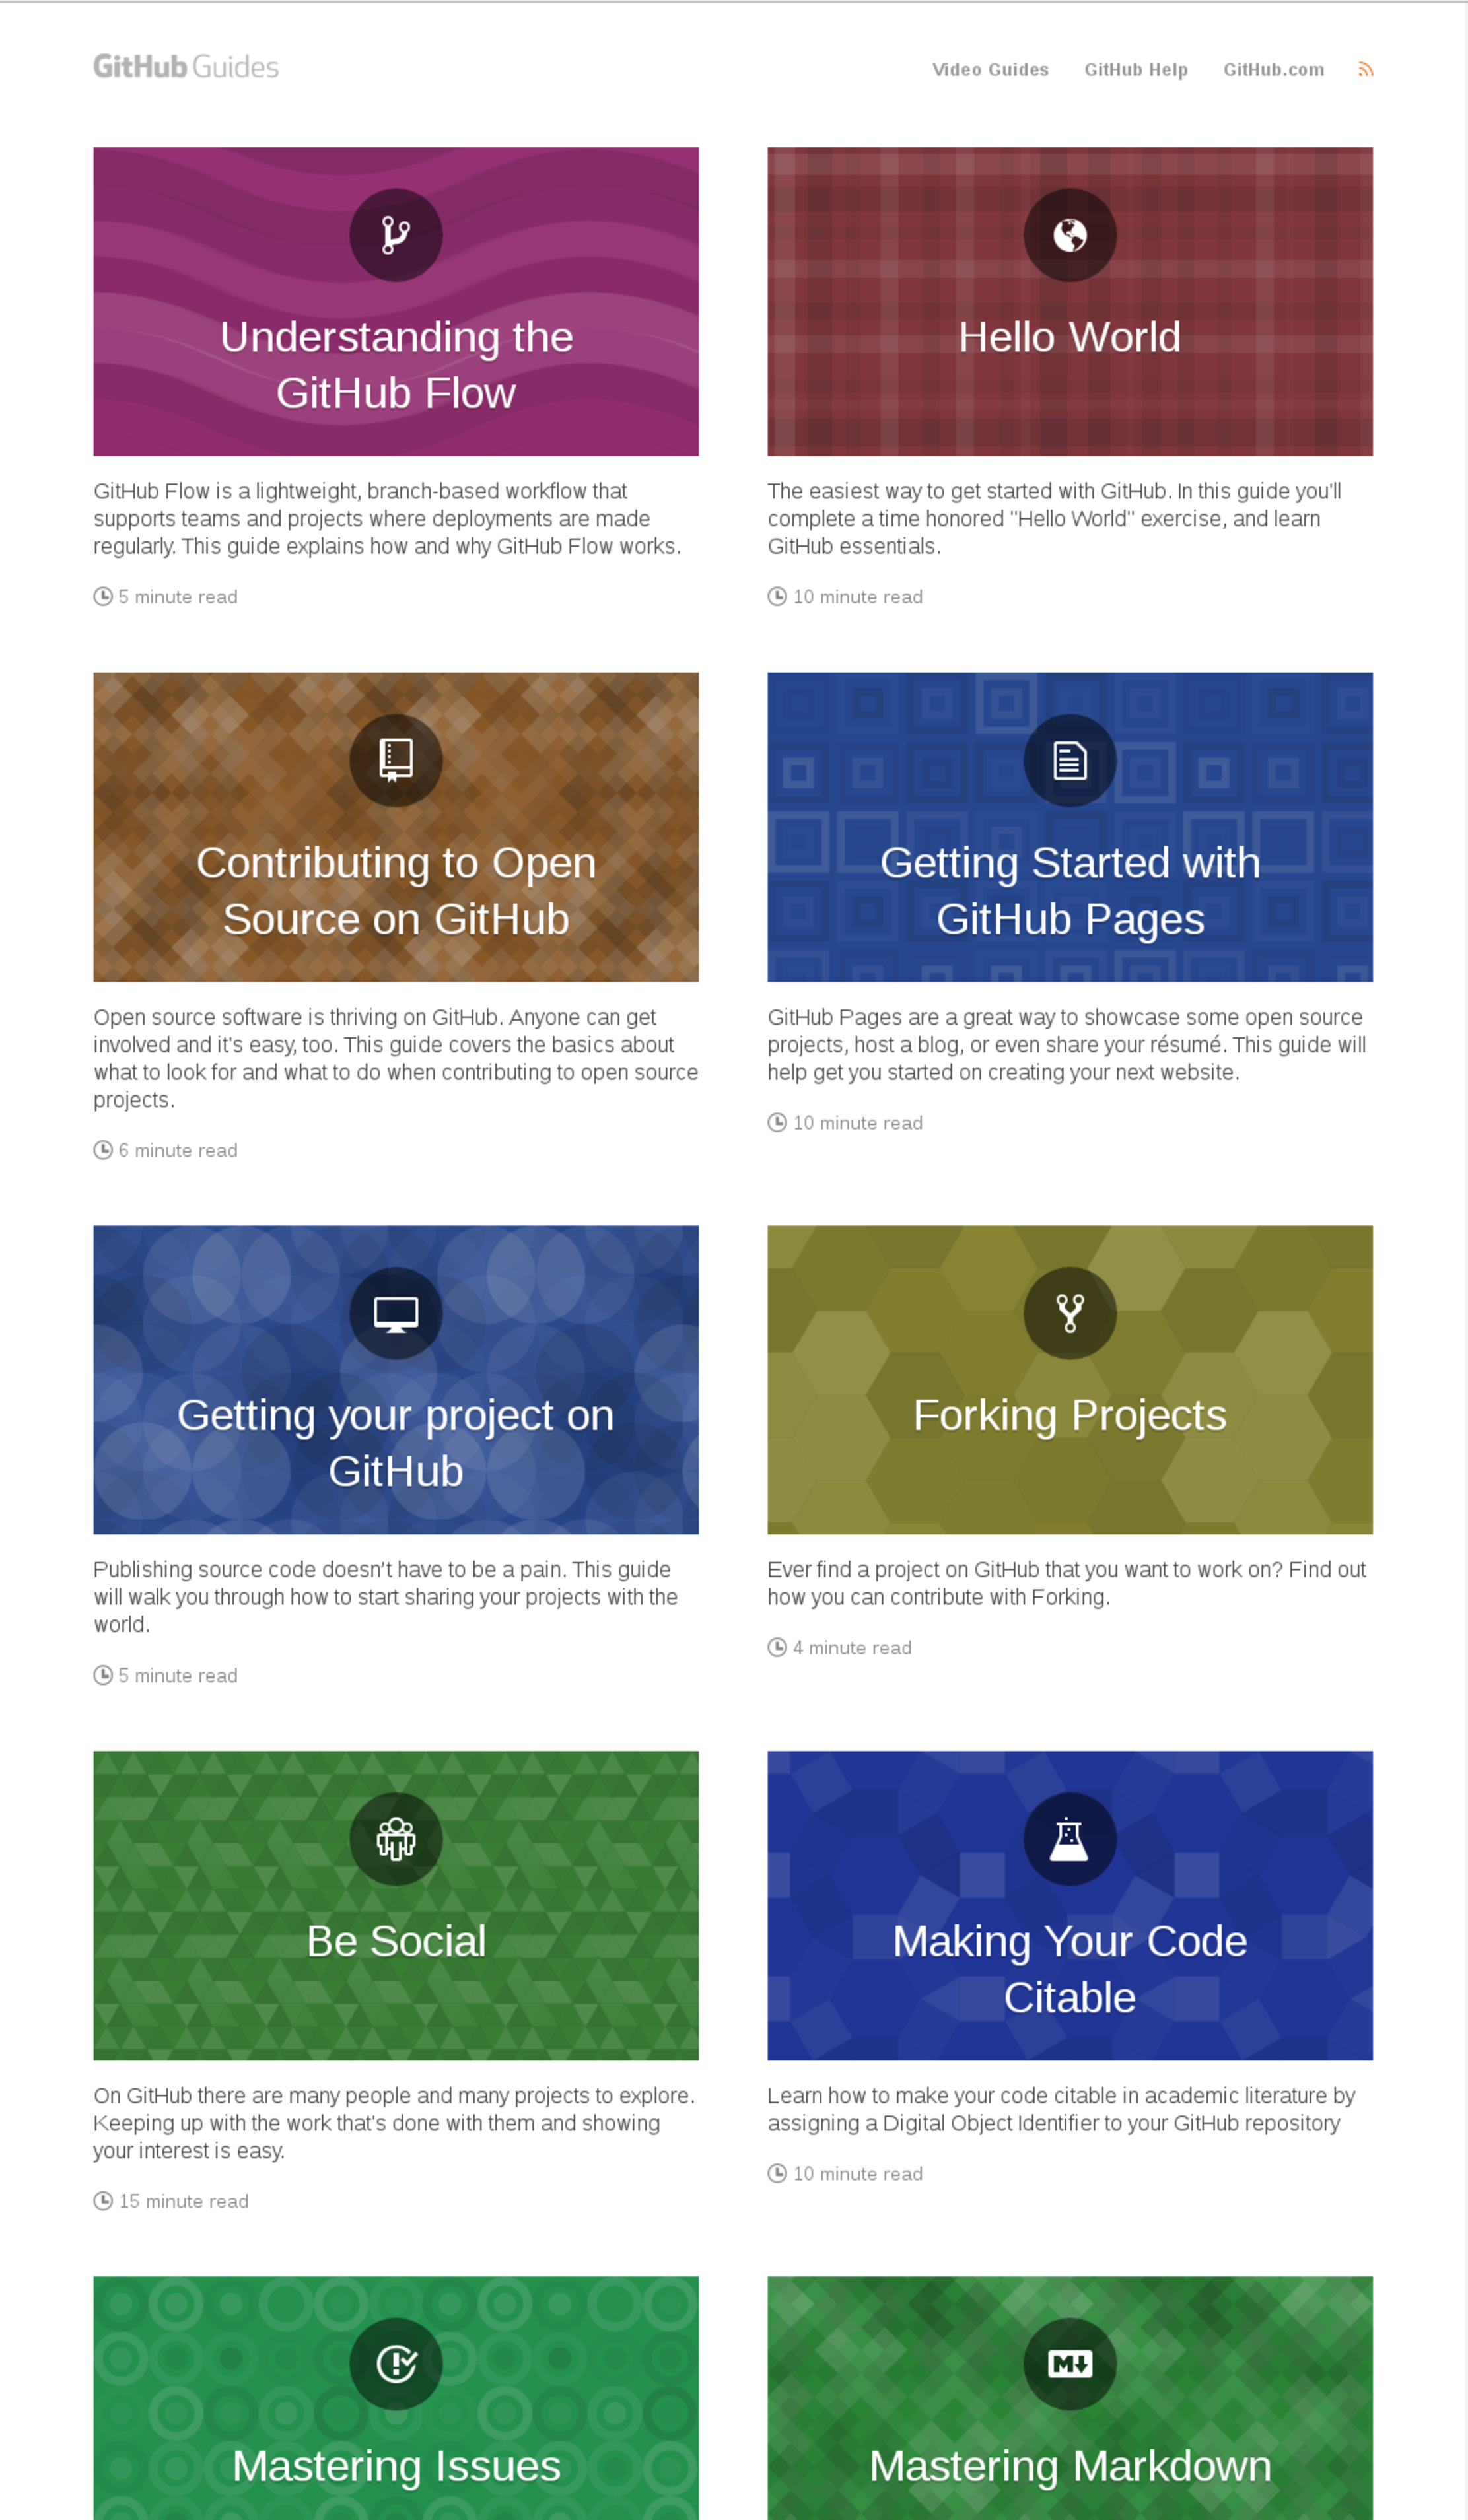
\includegraphics[trim = 0mm 375mm 0mm 0mm, clip = TRUE, width = \textwidth]{/home/ben/Intro_to_R/GitHub_Slides_Source/Images/Git_Resources/GitHub_Guides.pdf}
\end{figure}
\end{center}
\end{frame}

\begin{frame}
\frametitle{Recommended Further Reading}
\framesubtitle{\url{https://www.atlassian.com/git/tutorials/}}
\begin{center}
\begin{figure}

%trim option's parameter order: left bottom right top
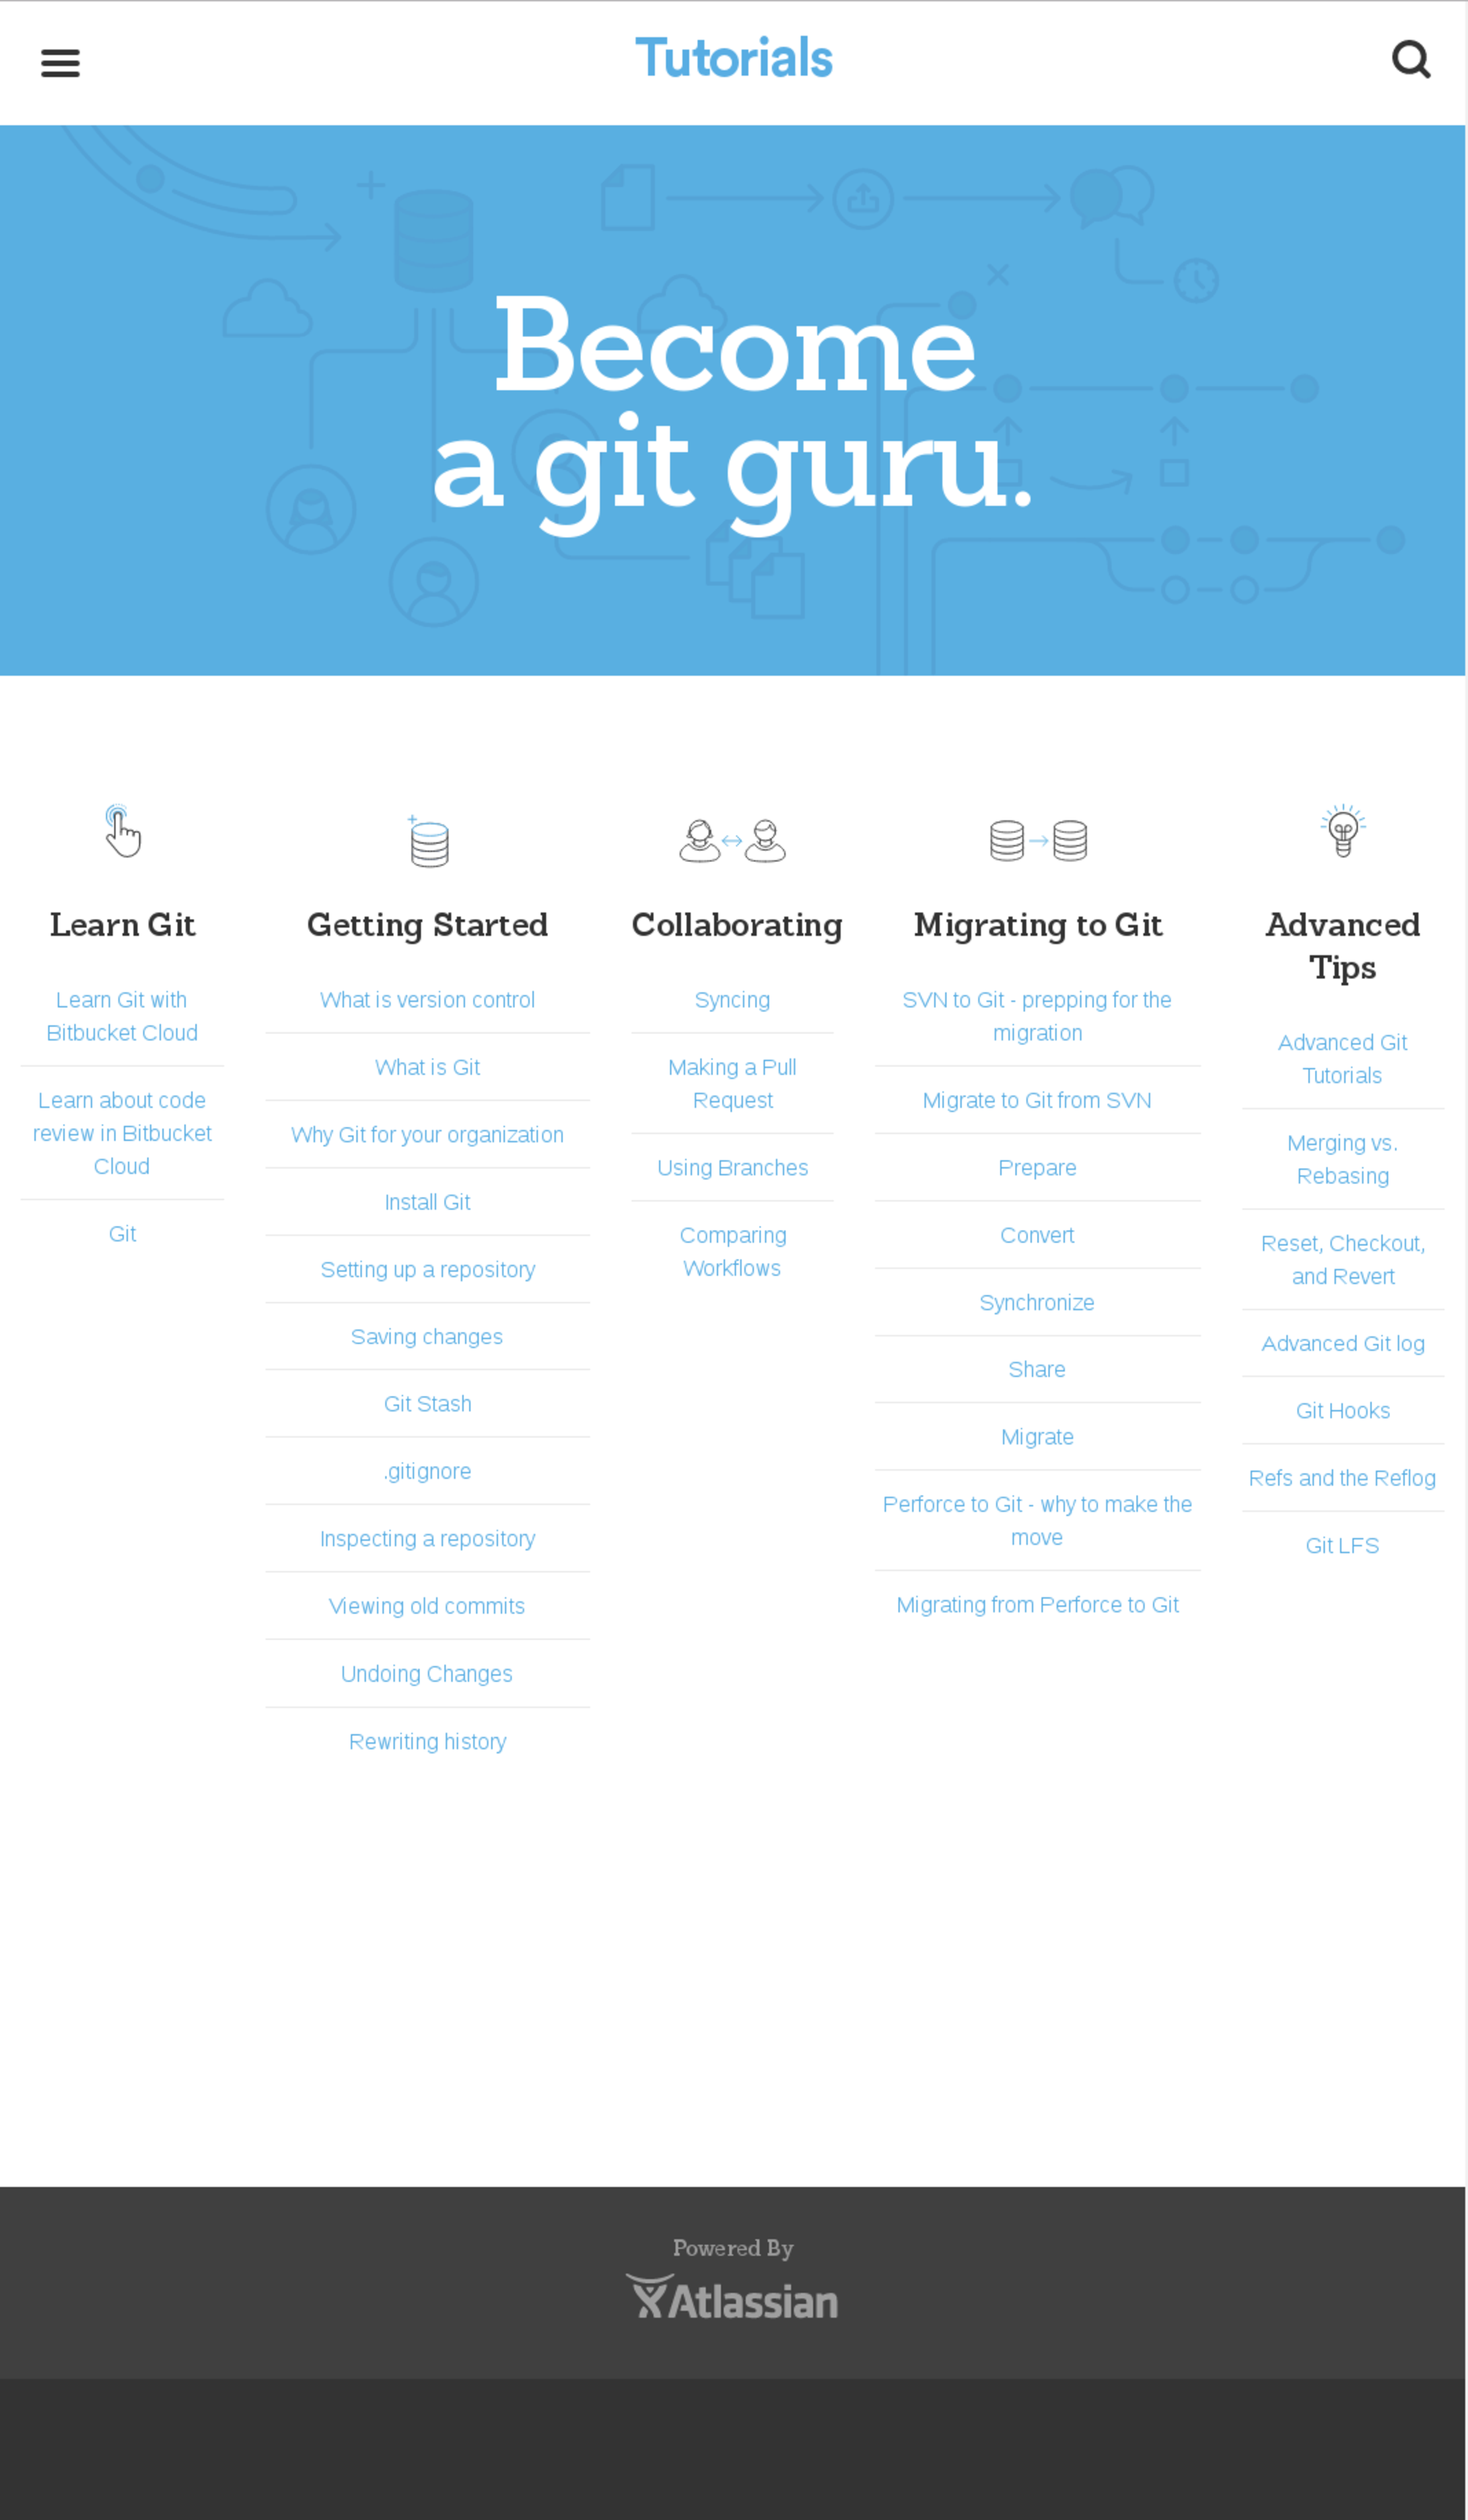
\includegraphics[trim = 0mm 375mm 0mm 0mm, clip = TRUE, width = \textwidth]{/home/ben/Intro_to_R/GitHub_Slides_Source/Images/Git_Resources/Atlassian_Tutorials.pdf}
\end{figure}
\end{center}
\end{frame}

\begin{frame}
\frametitle{Recommended Further Reading:}
\framesubtitle{\url{https://help.github.com/}}
%
\begin{center}
\begin{figure}
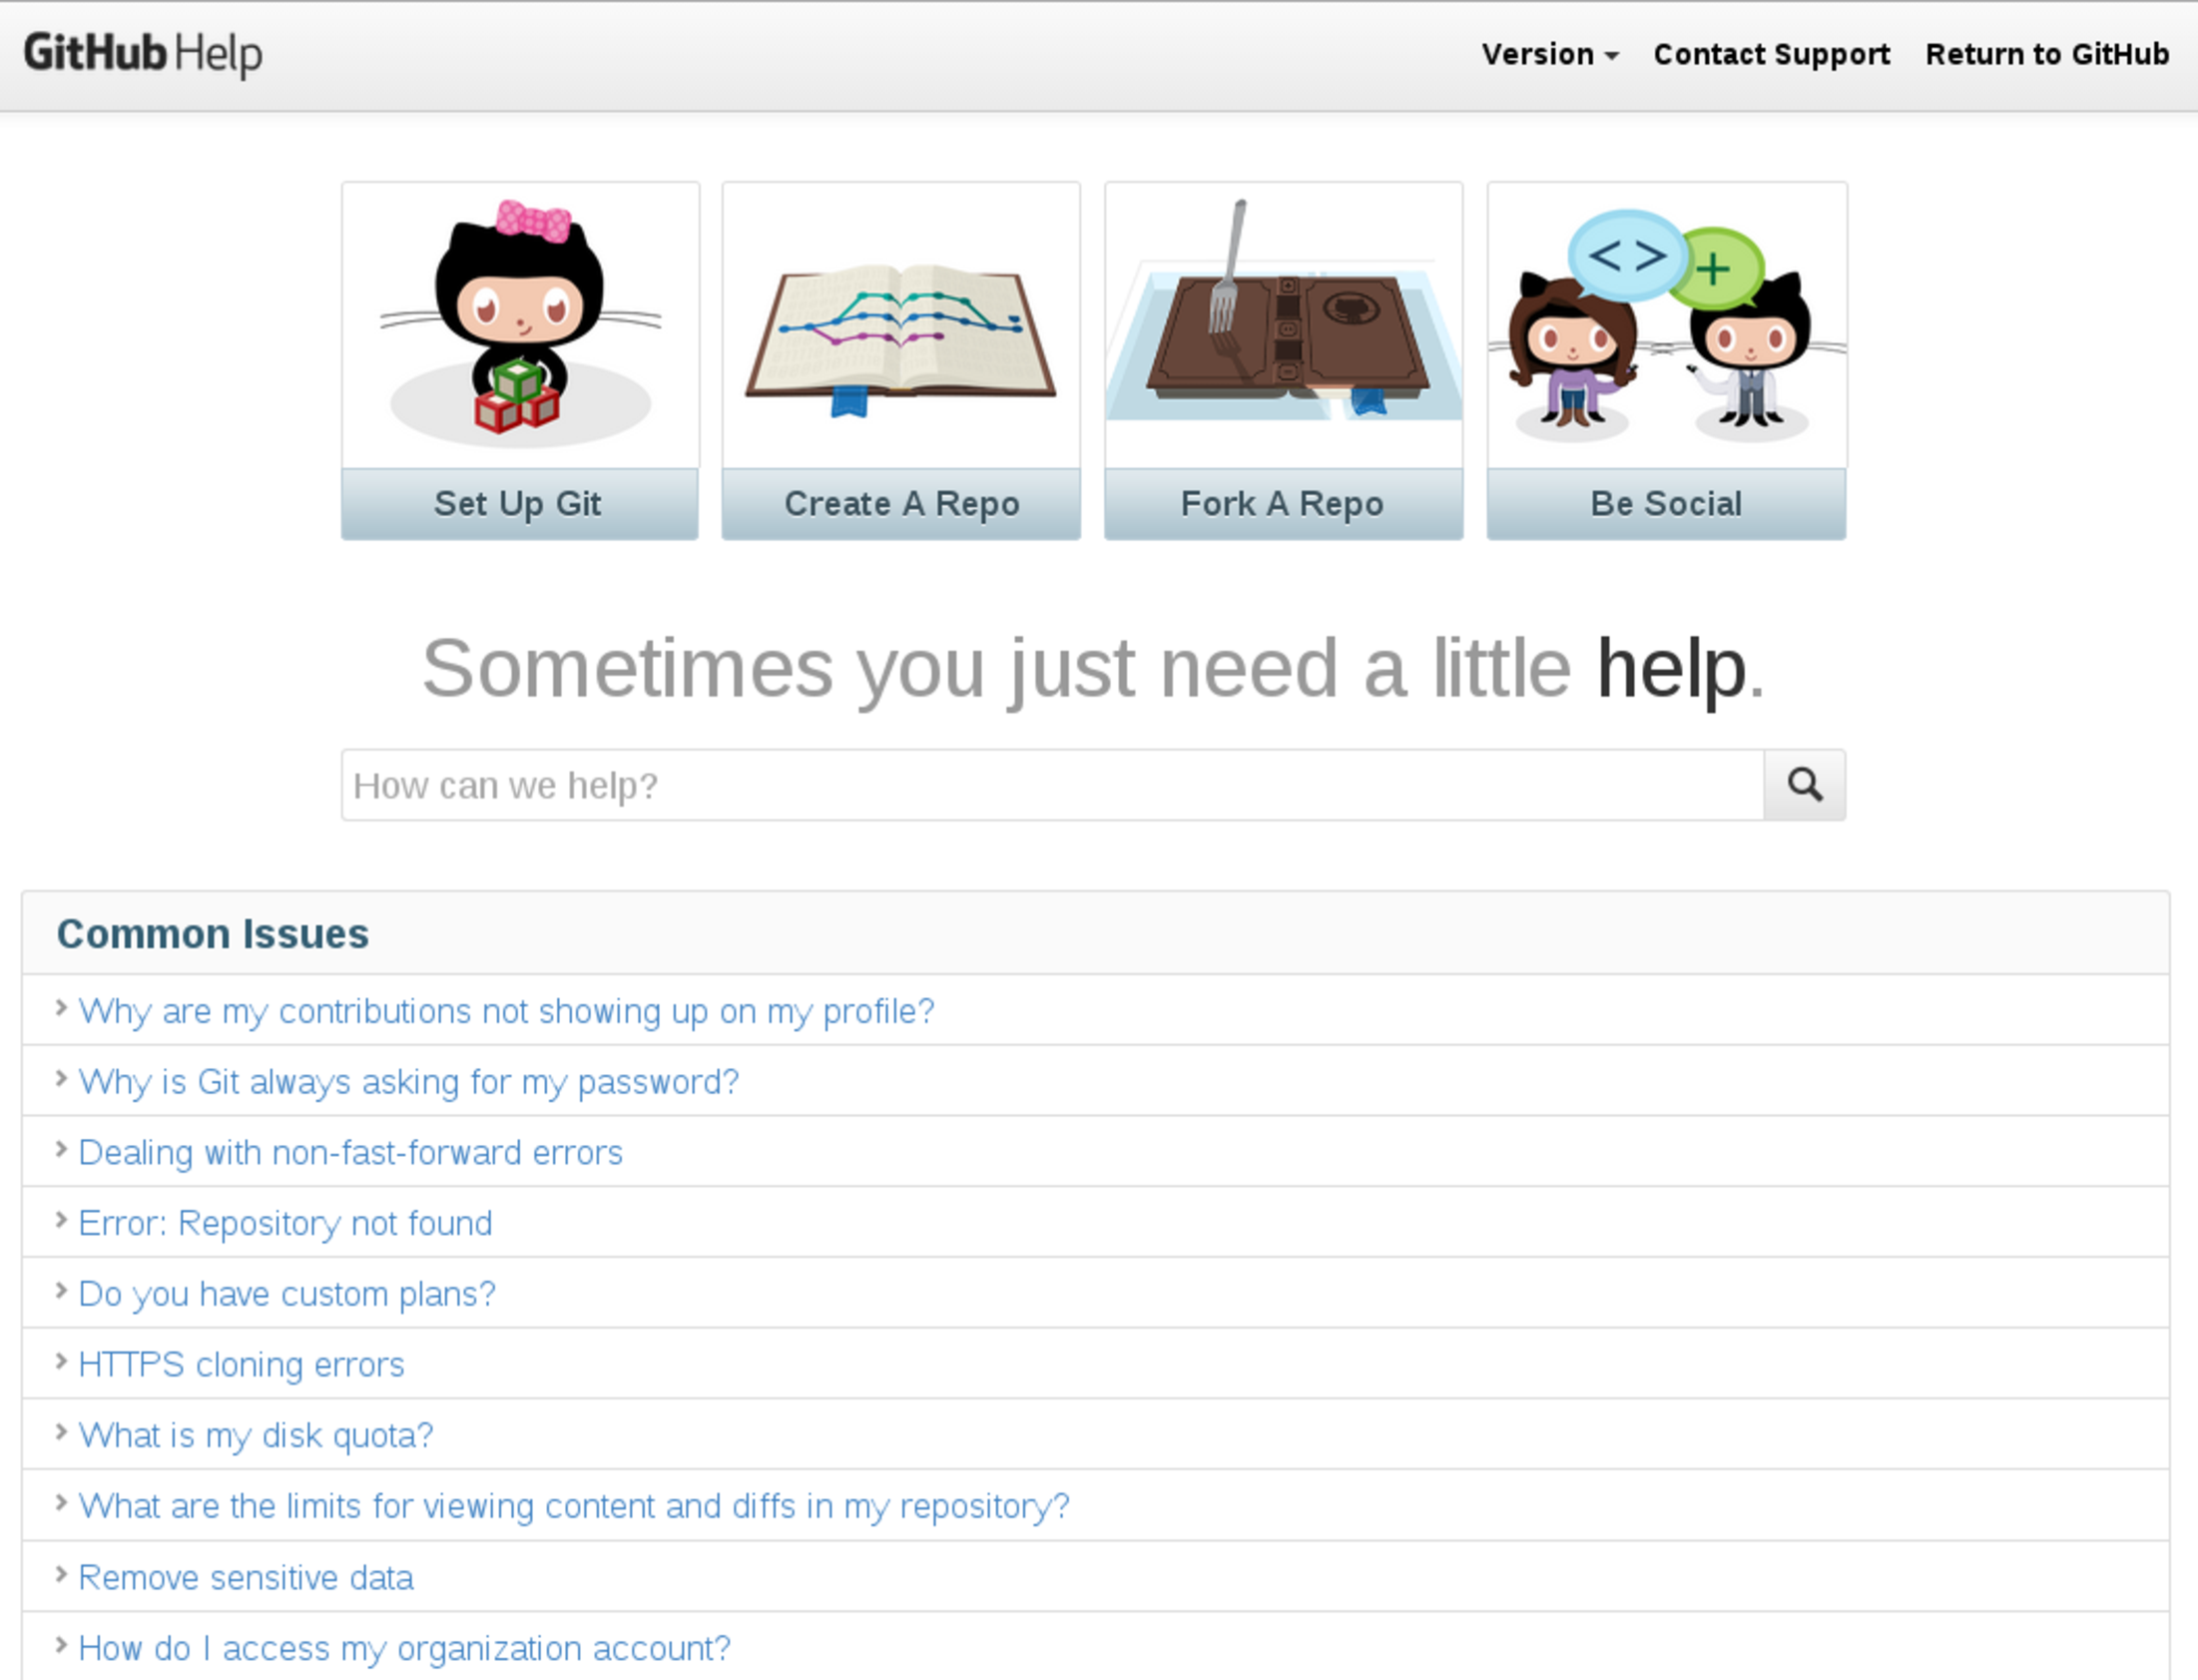
\includegraphics[width = 0.95\textwidth]{/home/ben/Intro_to_R/GitHub_Slides_Source/Images/Git_Resources/GitHub_Help_Page.pdf}
\end{figure}

\end{center}

\end{frame}

\begin{frame}
\frametitle{Image Credits}
\begin{itemize}
\item Git Logo by Jason Long \url{http://git-scm.com/downloads/logos}
\item GitHub Logo, \url{www.github.com}
\item R Logo, \url{www.r-project.org}
\end{itemize}
\end{frame}

\end{document}
